\documentclass{report}

\title{\huge 基础数据结构选讲}
\author{李昊泽}
\date{2025年10月7日}

\usepackage{ctex}
\usepackage{amsmath}
\usepackage{amssymb}
\usepackage{graphicx}
\usepackage{booktabs}
\usepackage[colorlinks=true]{hyperref}
\usepackage{geometry}
\usepackage{xcolor}
\usepackage{minted}

\setCJKmainfont{Noto Serif CJK SC}
\setCJKsansfont{Noto Sans CJK SC}

\setmonofont{Fira Code}
\setminted{
    fontsize    = \fontsize{8}{9.6}\selectfont,
    frame       = single,
    linenos     = true,
    breaklines  = true,
    breakanywhere = true,
    autogobble  = true
}

\geometry{a4paper, margin=2.5cm}

\begin{document}

\maketitle

\newpage

\tableofcontents

\newpage

\chapter{栈}

\section{引入}

\subsection{洗碗问题}

小泽是餐厅里的洗碗工。

每天都有堆积如山的盘子需要他洗。他每次从这叠盘子里面取出最顶上的那一个,然后把它洗干净,放到别的地方。

恰饭的人源源不断,所以需要洗的盘子也源源不断地送过来。每次来了新的盘子,都会被放在那叠盘子的最顶上。

\textbf{如何用一个数组模拟这叠盘子?}

\begin{figure}[ht]
    \centering
    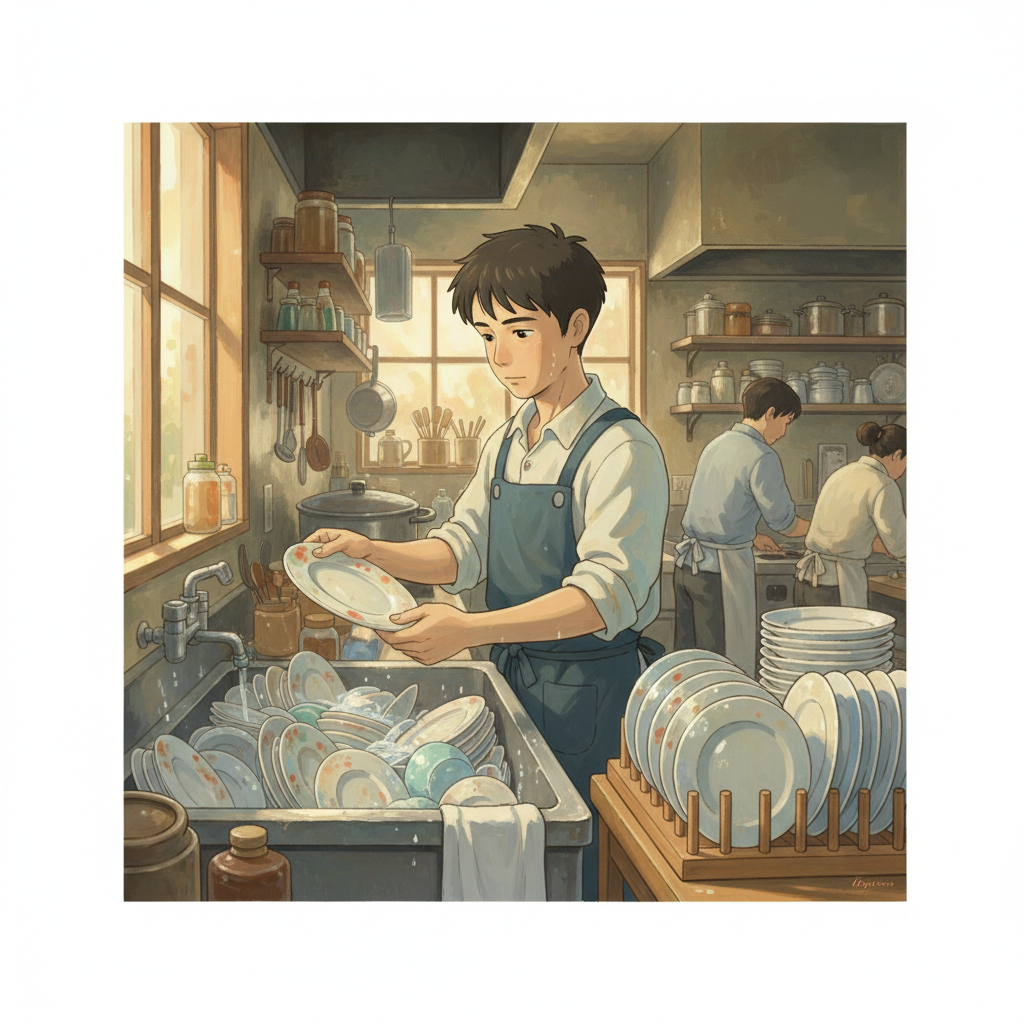
\includegraphics[width=0.5\textwidth]{./pic/Gemini_Generated_Image_4uekal4uekal4uek.png}
    \caption{洗碗示意图}
\end{figure}

\begin{table}[ht]
    \centering
    \begin{tabular}{cc}
        \toprule
        事件          & 状态    \\
        \midrule
        放入 1        & 1       \\
        放入 2        & 1, 2    \\
        放入 3        & 1, 2, 3 \\
        取出顶端(3) & 1, 2    \\
        取出顶端(2) & 1       \\
        放入 4        & 1, 4    \\
        放入 5        & 1, 4, 5 \\
        取出顶端(5) & 1, 4    \\
        取出顶端(4) & 1       \\
        取出顶端(1) & 空      \\
        \bottomrule
    \end{tabular}
    \caption{盘子操作状态变化}
\end{table}

\section{栈的性质}

在前面的引用中,我们发现:盘子都是从顶端进,从顶端出。如果 $a$ 比 $b$ 早进入,那么 $a$ 一定比 $b$ 后退出。

这个性质即为“后进先出”,它是 \textcolor{red}{栈} 的本质。

\textbf{栈}(stack):LIFO(Last In, First out)表

\section{栈的实现}

\subsection{C-style 模拟}

\begin{minted}{cpp}
int stk[N], top = 0;
// 向栈顶插入一个数
stk[++top] = x;
// 从栈顶弹出一个数
top--;
// 获取栈顶的值
stk[top];
// 判断栈是否为空
if (top > 0) { }
\end{minted}

\subsection{STL 实现}

STL 中可以使用 \texttt{std::vector} 来模拟栈操作,主要函数包括:

\begin{enumerate}
    \item 元素访问
    \begin{enumerate}
        \item \texttt{stk.back()} 返回栈顶元素
    \end{enumerate}
    \item 修改
    \begin{enumerate}
        \item \texttt{stk.push\_back()} 在栈顶插入元素
        \item \texttt{stk.pop\_back()} 弹出栈顶元素
    \end{enumerate}
    \item 容量
    \begin{enumerate}
        \item \texttt{stk.empty()} 栈是否为空
        \item \texttt{stk.size()} 返回栈中元素的数量
    \end{enumerate}
\end{enumerate}

\begin{minted}{cpp}
std::vector<int> stk;
// 向栈顶插入一个数
stk.push_back(x);
// 从栈顶弹出一个数
stk.pop_back();
// 获取栈顶的值
stk.back();
// 判断栈是否为空
if (!stk.empty()) { }
\end{minted}

\section{例题}

\subsection{例题一 \ 栈的实现}

请你实现一个栈(stack),支持以下操作:

\begin{enumerate}
    \item \texttt{push(x)}: 向栈中加入一个数 x。
    \item \texttt{pop()}: 将栈顶输出。如果此时栈为空则不进行弹出操作,输出 \texttt{Empty}。
    \item \texttt{query()}: 输出栈顶元素,如果此时栈为空则输出 \texttt{Anguei!}。
    \item \texttt{size()}: 输出此时栈内元素个数。
\end{enumerate}

\subsubsection{代码}

此处使用 \texttt{std::vector} 进行栈的模拟。

以下仅展示核心逻辑部分的代码。

\begin{minted}{cpp}
if (op == "push") {
    u64 x;
    std::cin >> x;
    stk.push_back(x);
} else if (op == "pop") {
    if (stk.empty()) {
        std::cout << "Empty\n";
    } else {
        stk.pop_back();
    }
} else if (op == "query") {
    if (stk.empty()) {
        std::cout << "Anguei!\n";
    } else {
        std::cout << stk.back() << "\n";
    }
} else {
    std::cout << stk.size() << "\n";
}
\end{minted}

\subsection{例题二 \ 括号匹配问题}

给定一串由 () 和 [] 组成的字符串,我们规定以下的字符串是合法的字符串:

\begin{enumerate}
    \item 空串是合法的
    \item 如果 A、B 都是合法的,那么 AB 是合法的
    \item 如果 A 是合法的,那么 (A) 和 [A] 都是合法的
\end{enumerate}

请写出一个程序,判断每一个给定的字符串是否合法。

\subsubsection{分析}

我们可以先手玩一下以下的字符串是否合法:

\begin{itemize}
    \item \texttt{[(())]}
    \item \texttt{()[]()}
    \item \texttt{[([])[]]()}
    \item \texttt{(()}
    \item \texttt{([)(])}
\end{itemize}

将一个字符串从左往右写,一旦遇到匹配上的括号,就把这对括号擦掉。

我们可以使用一个栈来维护上面的操作。

当新加入一个括号时:

\begin{enumerate}
    \item 如果是左括号,则把这个括号入栈
    \item 如果是右括号,看栈顶是否能和这个右括号匹配,如果可以的话弹出栈顶,否则这个字符串不合法
\end{enumerate}

\subsubsection{代码}

完整代码见 \href{https://vjudge.net/solution/64150195/NWv7brPjI5uhjS91FLfu}{vjudge 提交记录}

\begin{minted}{cpp}
for (int i = 0; i < s.length(); i++) {
    if (s[i] == '(' or s[i] == '[') {
        stk.push_back(s[i]);
    } else {
        if (not stk.empty() and s[i] == ')' and stk.back() == '(') {
            stk.pop_back();
        } else if (not stk.empty() and s[i] == ']' and stk.back() == '[') {
            stk.pop_back();
        } else {
            std::cout << "No\n";
            return;
        }
    }
}
if (not stk.empty()) {
    std::cout << "No\n";
} else {
    std::cout << "Yes\n";
}
\end{minted}

\subsection{例题三 \ 后缀表达式}

所谓后缀表达式是指这样的一个表达式:式中不再引用括号,运算符号放在两个运算对象之后,所有计算按运算符号出现的顺序,严格地由左而右新进行(不用考虑运算符的优先级)。

本题中运算符仅包含 $+ - * /$。保证对于 $/$ 运算除数不为 $0$。特别地,其中 $/$ 运算的结果需要向 $0$ 取整(即与 C++ $/$ 运算的规则一致)。

如:$3*(5-2)+7$ 对应的后缀表达式为:$3.5.2.-*7.+@$。在该式中,$@$ 为表达式的结束符号。$.$ 为操作数的结束符号。

\subsubsection{分析}

后缀表达式不需要使用括号,其运算方案是唯一的。对于计算机来说,最容易理解后缀表达式。

\begin{center}
    \fbox{
        \parbox{\textwidth}{
            \centering
            \textbf{后缀表达式求值}

            \begin{enumerate}
                \item 建立一个用于存数的栈,逐一扫描该后缀表达式中的元素。
                \begin{enumerate}
                    \item 如果遇到一个数,则把该数入栈
                    \item 如果遇到运算符,就取出栈顶的两个数进行计算,把结果入栈
                \end{enumerate}
                \item 扫描完成后,栈中恰好剩下一个数,就是该后缀表达式的值
            \end{enumerate}
        }
    }
\end{center}

\subsubsection{代码}

由于该题的逆天输入格式,这里使用 Java 代码演示主要逻辑:

\begin{minted}{java}
Pattern p = Pattern.compile("(\\d+|[+\\-*\\/])");
Matcher m = p.matcher(s);

Stack<Integer> stk = new Stack<>();
while (m.find()) {
    String x = m.group(1);
    if (x.matches("\\d+")) {
        stk.push(Integer.parseInt(x));
    } else {
        int b = stk.peek();
        stk.pop();
        int a = stk.peek();
        stk.pop();
        stk.push(
            switch (x) {
                case "+" -> a + b;
                case "-" -> a - b;
                case "*" -> a * b;
                case "/" -> a / b;
                default -> 0;
            }
        );
    }
}
System.out.println(stk.peek());
\end{minted}

\section{课后作业}

\begin{itemize}
    \item 最小栈 \href{https://leetcode.cn/problems/min-stack/}{LeetCode 155} (栈的灵活应用)
    \item Editor \href{https://acm.hdu.edu.cn/showproblem.php?pid=4699}{HDU 4699}(对顶栈)
    \item \string[NOIP 2013 普及组\string] 表达式求值 \href{https://www.luogu.com.cn/problem/P1981}{Luogu P1981} (中缀表达式求值)
    \item \string[河南省第十五届ICPC大学生程序设计竞赛\string] 表达式求导 (中缀表达式递归求值)
    \item \string[NOIP 2003 普及组] 栈 \href{https://www.luogu.com.cn/problem/P1044}{Luogu P1044} (栈的数学性质)
\end{itemize}

\section{进阶:单调栈}

顾名思义,单调栈即满足单调性的栈结构。

常用于找出每个数左边离它最近的比它大/小的数,也可用于求出"以某个只为最值的最大区间"。

是较为常用的优化技巧,借助单调性处理问题,\textbf{及时排除不可能的选项,保持策略集合的高度有序性和秩序性}。

\subsection{例题}

\subsubsection{例题一 \ 单调栈}

给出项数为 $n$ 的整数数列 $a_{1 \dots n}$。

定义函数 $f(i)$ 代表数列中第 $i$ 个元素之后第一个大于 $a_i$ 的元素的\textbf{下标},即
$f(i)=\min_{i<j\leq n, a_j > a_i} \{j\}$
若不存在,则 $f(i)=0$。

试求出 $f(1\dots n)$。

\paragraph{代码}

\begin{minted}{cpp}
std::vector<int> ans(n);
std::vector<int> stk;
for (int i = n - 1; i >= 0; i--) {
    while (not stk.empty() and a[stk.back()] <= a[i]) {
        stk.pop_back();
    }
    if (stk.empty()) {
        ans[i] = -1;
    } else {
        ans[i] = stk.back();
    }
    stk.push_back(i);
}

for (int i = 0; i < n; i++) {
    std::cout << ans[i] + 1 << " \n"[i == n - 1];
}
\end{minted}

\subsubsection{例题二 Largest Rectangle in a Histogram}

如下图所示,在一条水平线上方有若干个矩形,求包含与这些矩形的并集内部的最大矩形的面积。(在下图中,答案就是阴影部分的面积),矩形个数 $\le 10^5$。

\begin{figure}[ht]
    \centering
    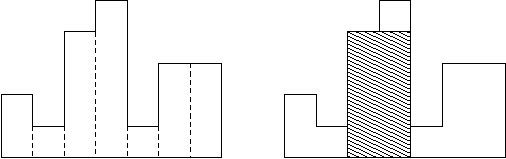
\includegraphics[width=0.5\textwidth]{./pic/rectangle.png}
    \caption{直方图最大矩形}
\end{figure}

\paragraph{分析}

我们考虑简化的问题:如果矩形的高度从左到右单调递加,那么答案怎么计算?显然局部最优解是每个矩形的高度作为最终矩形的高度,宽度延伸到右边界,在所有这样的矩形中取最大值就是答案。

如果下一个矩形的高度比上一个小,那么之前高出来的部分就不能利用了,我们可以把这些矩形删掉,用一个合并过的新矩形代替,不会影响后面的计算。

于是我们维护的轮廓就变成了一个高度始终单调递增的矩形序列,我们可以添加一个高度为 $0$ 的虚拟矩形,避免扫描结束后栈中有剩余矩形。

\paragraph{代码}

\begin{minted}{cpp}
std::vector<int> h(n + 1), w(n + 1);
for (int i = 0; i < n; i++) {
    std::cin >> h[i];
}

i64 ans = 0;
std::vector<int> stk;
for (int i = 0; i <= n; i++) {
    while (!stk.empty() && h[stk.back()] > h[i]) {
        w[i] += w[stk.back()];
        ans = std::max(ans, 1LL * w[i] * h[stk.back()]);
        stk.pop_back();
    }
    w[i]++;
    stk.push_back(i);
}
std::cout << ans << "\n";
\end{minted}

\newpage

\chapter{队列}

\section{引入}

\subsection{排队问题}

这回小泽作为一个收银员在超市打工。收银员会给排在队伍最前面的顾客结账,然后服务队伍中的下一个顾客。而队伍的末尾也一直会有更多的顾客依次加人队列。

如何用一个数组模拟这个队伍?

\begin{figure}[H]
    \centering
    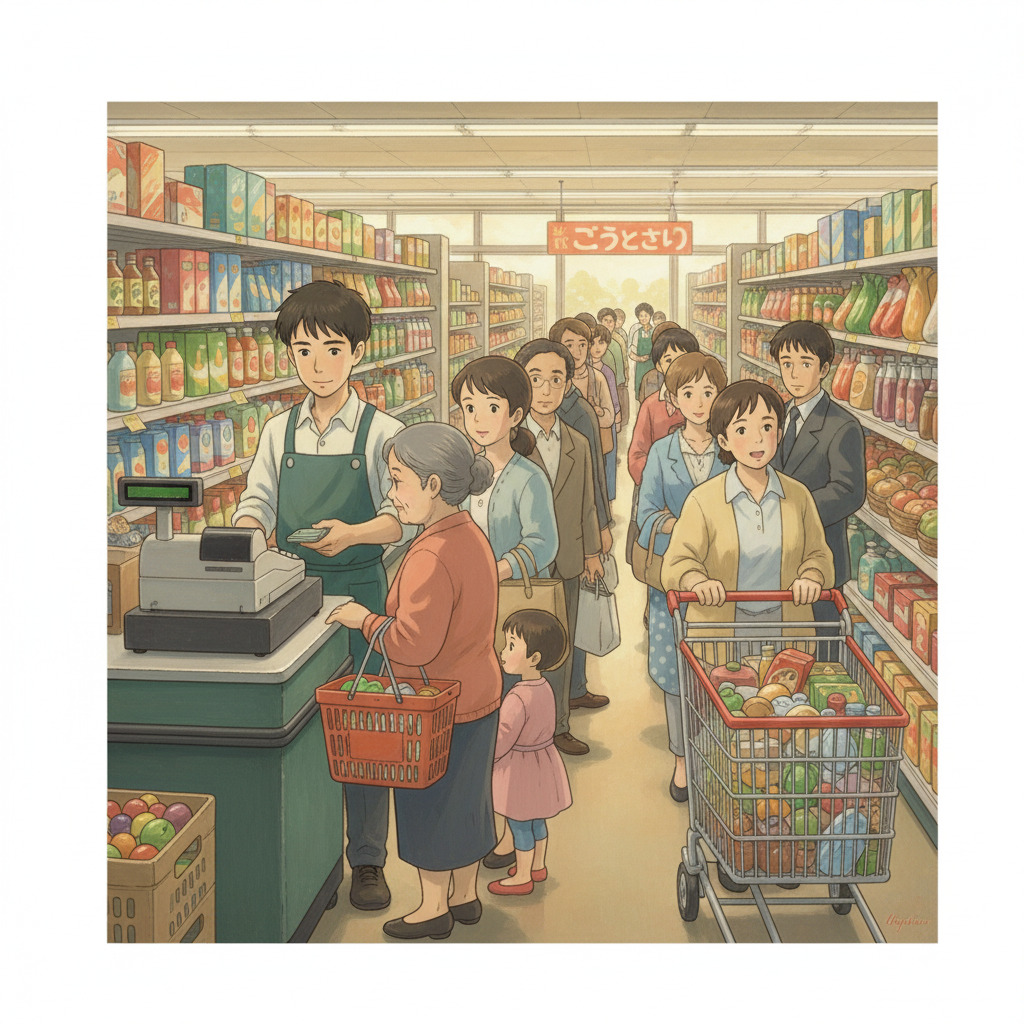
\includegraphics[width=0.5\textwidth]{./pic/Gemini_Generated_Image_2sj2u2sj2u2sj2u2.png}
    \caption{小泽收银图}
\end{figure}

\begin{table}[ht]
    \centering
    \begin{tabular}{@{}ll@{}}
        \toprule
        事件              & 队伍的状态 \\
        \midrule
        顾客1加入队列     & 1          \\
        顾客2加入队列     & 1 2        \\
        顾客3加入队列     & 1 2 3      \\
        收银员帮顾客1买单 & 2 3        \\
        收银员帮顾客2买单 & 3          \\
        顾客4加入队列     & 2 4        \\
        顾客5加入队列     & 3 4 5      \\
        收银员帮顾客3买单 & 4 5        \\
        收银员帮顾客4买单 & 5          \\
        收银员帮顾客5买单 & 空         \\
        \bottomrule
    \end{tabular}
    \caption{队列操作状态变化}
\end{table}

\section{队列的性质}

\textcolor{red}{队列}的本质是"先进先出":越先来的,越早办完事。

\textbf{队列}(queue):FIFO(First In, First Out)表。

\section{队列的实现}

\subsection{C-style 模拟}

\begin{minted}{cpp}
int q[N], head = 0, tail = -1;
// 向队列中加入一个数
q[++tail] = x;
// 从队头弹出一个数
head++;
// 获取队头的值
q[head];
// 判断队列是否为空
if (head <= tail) { }
\end{minted}

\subsection{循环队列}

我们发现,当弹出较多元素时,数组中队头之前的空间就浪费了,\textbf{循环队列} 是一种充分利用数组空间的方法。

\begin{minted}{cpp}
int q[N], head = 0, tail = 0;
// 向队列中加入一个数
q[tail++] = x;
if (tail == N) {
    tail = 0;
}
// 从队头弹出一个数
head++;
if (head == N) {
    head = 0;
}
// 获取队头的值
q[head];
// 判断队列是否为空
if (head != tail) { }
\end{minted}

\subsection{STL 实现}

STL 中的 \texttt{std::queue} 容器提供了一众成员函数一共调用,其中常用操作有:

\begin{enumerate}
    \item 元素访问
    \begin{enumerate}
        \item \texttt{q.front()} 返回队首元素
        \item \texttt{q.back()} 返回队尾元素
    \end{enumerate}
    \item 修改
    \begin{enumerate}
        \item \texttt{q.push()} 在队尾插入元素
        \item \texttt{q.pop()} 弹出队首元素
    \end{enumerate}
    \item 容量
    \begin{enumerate}
        \item \texttt{q.empty()} 队列是否为空
        \item \texttt{q.size()} 返回队列中元素的数量
    \end{enumerate}
\end{enumerate}

双端队列 \texttt{std::deque} 的操作相似。

\section{例题}

\subsection{例题一 \ 约瑟夫问题}

$n$ 个人围成一圈,从第一个人开始报数,数到 $m$ 的人出列,再由下一个人重新从 $1$ 开始报数,数到 $m$ 的人再出圈,依次类推,直到所有的人都出圈,请输出依次出圈人的编号。

\subsubsection{代码}

由于每个小朋友都有机会数 $m$ 次,所以时间复杂度是 $O(nm)$。

\begin{minted}{cpp}
std::queue<int> q;
for (int i = 1; i <= n; i++) {
    q.push(i);
}

int cur = 1;
while (not q.empty()) {
    int x = q.front();
    q.pop();

    if (cur != m) {
        q.push(x);
        cur++;
    } else {
        std::cout << x << " ";
        cur = 1;
    }
}
\end{minted}

\section{课后作业}

\begin{itemize}
    \item \string[NOIP 2010 提高组\string] 机器翻译 \href{https://www.luogu.com.cn/problem/P1540}{Luogu P1540} (队列的应用)
\end{itemize}

\section{进阶:单调队列}

单调队列的思想和单调栈相同,\textbf{在决策集合中及时排除一定不是最优解的选择}。

在 OI 圈中有一句生动形象的话来形容其原理:"*如果一个选手比你小还比你强,那你就可以退役了*",这启发我们用贡献的角度考虑其原理:更老而更弱的选手贡献更小。

单调队列是一种优化动态规划的重要手段。

\subsection{例题一 \ 扫描}

有一个 $1 \times n$ 的矩阵,有 $n$ 个整数。

现在给你一个可以盖住连续 $k$ 个数的木板。

一开始木板盖住了矩阵的第 $1 \sim k$ 个数,每次将木板向右移动一个单位,直到右端与第 $n$ 个数重合。

每次移动前输出被覆盖住的数字中最大的数是多少。

\subsubsection{分析}

这是一道\textbf{滑动窗口}的裸题,我们先手玩一下样例:

\begin{verbatim}
5 3
1 5 3 4 2
\end{verbatim}

过程如下:
\[
\begin{aligned}
	& \underline{1 \ \boxed{5} \ 3} \ 4 \ 2 \\
	& 1 \ \underline{\boxed{5} \ 3 \ 4} \ 2 \\
	& 1 \ 5 \ \underline{3 \ \boxed{4} \ 2}
\end{aligned}
\]

如果用最暴力的 $O(n k)$ 做法,显然进行了大量的重复工作:一个更靠前但更小的数显然对答案没有贡献(更老但是更弱的选手可以退役了)。

我们可以维护一个长度有限的队列,其内部\textbf{索引递增,数值递减},队头即为当前的最大值。

当队头的索引超出范围时,弹出队头,维护区间的长度。

当新加一个数的时候,我们把队尾所有小于当前数的元素删掉,从而维护单调性。

由于每一个数最多\textbf{入队一次,出队一次},所以算法的时间复杂度是 $O(n)$。

\newpage

\subsubsection{代码}

\begin{minted}{cpp}
std::vector<int> ans(n);
std::deque<int> q;
for (int i = 0; i < n; i++) {
    if (not q.empty() and q.front() < i - k + 1) {
        q.pop_front();
    }
    while (not q.empty() and a[q.back()] < a[i]) {
        q.pop_back();
    }
    q.push_back(i);
    ans[i] = a[q.front()];
}
for (int i = k - 1; i < n; i++) {
    std::cout << ans[i] << "\n";
}
\end{minted}

\subsection{例题二 \ 最大子序和}

输入一个长度为 $n$ 的整数序列(可能有负数),从中找出一段长度不超过 $m$ 的连续子序列,使得子序列中所有数的和最大。

\subsubsection{分析}

我们知道,区间和问题可以使用前缀和求解:连续子序列 $[l, r]$ 中的数的和等于 $s[r] - s[l - 1]$。于是问题可以转化为:找出两个位置 $x, y$,使得 $s[y] - s[x]$ 最大,其中 $y - x \le m$。

对于一个固定的 $y$,问题转化为:找到一个左端点 $x \in [y - m, y - 1]$,使得 $s[x]$ 最小。

通过上面的分析,我们将该题转化为在一个长度固定的区间内找最小值的问题,即上面的\textbf{滑动窗口}问题。

\subsubsection{代码}

\begin{minted}{cpp}
i64 ans = -inf;
std::deque<int> q;
for (int i = 0; i <= n; i++) {
    if (not q.empty() and q.front() < i - m) {
        q.pop_front();
    }
    if (not q.empty()) {
        ans = std::max(ans, pre[i] - pre[q.front()]);
    }
    while (not q.empty() and pre[q.back()] > pre[i]) {
        q.pop_back();
    }
    q.push_back(i);
}
std::cout << ans << "\n";
\end{minted}

\chapter{链表}

\section{链表的性质}

数组是一种支持随机访问,但不支持在任意位置插入或删除元素的数据结构。与之对应,链表支持在任意位置插入或删除,但只能按顺序依次访问其中的元素。

\textcolor{red}{链表} 的本质是相邻元素相连接。

\section{链表的实现}

通常使用 C-style 数组模拟实现链表:

\begin{minted}{cpp}
// e[]表示节点的值,l[]表示节点的左指针,r[]表示节点的右指针,idx表示当前用到了哪个节点
int e[N], l[N], r[N], idx;
// 初始化
void init()
{
    //0是左端点,1是右端点
    r[0] = 1, l[1] = 0;
    idx = 2;
}
// 在节点a的右边插入一个数x
void insert(int a, int x)
{
    e[idx] = x;
    l[idx] = a, r[idx] = r[a];
    l[r[a]] = idx, r[a] = idx ++ ;
}
// 删除节点a
void remove(int a)
{
    l[r[a]] = l[a];
    r[l[a]] = r[a];
}
\end{minted}

\section{例题}

\subsection{例题一 \ 约瑟夫问题}

跟前面的问题相同,你能使用链表实现吗?

\subsection{例题二 \ 链式前向星}

读入 $n$ 个点,$m$ 条边,保存这个图。

\subsubsection{分析}

\textbf{邻接表}是链表的其中一个重要应用,它是树与图结构的一般化存储方式。

具体来说,链式前向星实现的邻接表,是用一个数组存每一个点的出边组成的链表的"表头"。

链式前向星中一般而言使用 $h, e, ne, w$ 四个数组来存图,$h$ 和 $ne$ 数组存的是 "$e$ 数组的下标",相当于指针。$e$ 数组存储的是每条边的终点,$w$ 数组存储的是每条边的权值,是图的真实数据。

我们使用 $h$ 获取"表头",$ne$ 获取当前边在出边组成的链表中的后继,进而可以遍历某个点的每一个出边。

\subsubsection{代码}

\begin{minted}{cpp}
// 对于每个点k,开一个单链表,存储k所有可以走到的点。h[k]存储这个单链表的头结点
int h[N], e[N], ne[N], idx;
// 添加一条边a->b
void add(int a, int b)
{
    e[idx] = b, ne[idx] = h[a], h[a] = idx ++ ;
}
// 初始化
idx = 0;
memset(h, -1, sizeof h);
// 遍历某个节点的所有出边
for (int i = h[u]; i != -1; i = ne[i]) { }
\end{minted}

\chapter{并查集 \& Hash 表(未完待续)}

\end{document}